\documentclass{article}

\usepackage{amsmath}
\usepackage[margin=1in]{geometry}
\usepackage{enumitem}
\usepackage{listings}
\usepackage{tikz}

\usetikzlibrary{automata,arrows,decorations.pathreplacing}

\tikzset{->,>=stealth',shorten >=1pt,auto,node distance=1.5cm,baseline={([yshift={-\ht\strutbox}]a.north)}}

\lstset
{language=C
,basicstyle=\footnotesize
,frame=single
}

\begin{document}
\title{Computation Theory -- supervision 1}
\author{James Wood}
\maketitle

\begin{enumerate}
  \item
    \begin{enumerate}[label=\arabic{enumii}.]
      \item
        \begin{enumerate}[label=(\alph{enumiii})]
          \item
            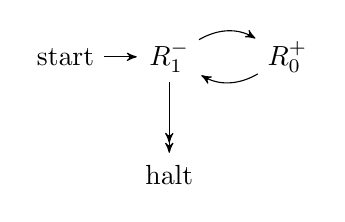
\begin{tikzpicture}
              \node[initial] (a) {$R_1^-$};
              \node (b) [right of=a] {$R_0^+$};
              \node (halt) [below of=a] {halt};

              \path
              (a) edge [bend left] (b)
              (b) edge [bend left] (a)
              (a) edge [->>] (halt)
              ;
            \end{tikzpicture}
          \item
            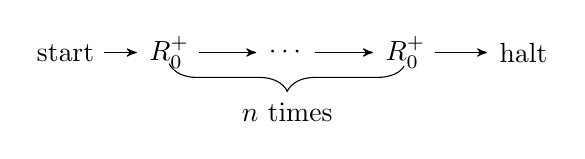
\begin{tikzpicture}
              \node[initial] (a) {$R_0^+$};
              \node (b) [right of=a] {$\cdots$};
              \node (c) [right of=b] {$R_0^+$};
              \node (halt) [right of=c] {halt};

              \path
              (a) edge (b)
              (b) edge (c)
              (c) edge (halt)
              ;

              \coordinate[left of=b] (al);
              \coordinate[right of=b] (cr);

              \draw[-,decorate,decoration={mirror,brace,amplitude=10pt,raise=4pt}] (al) -- (cr) node [midway,yshift=-1cm] {$n$ times};
            \end{tikzpicture}
          \item
            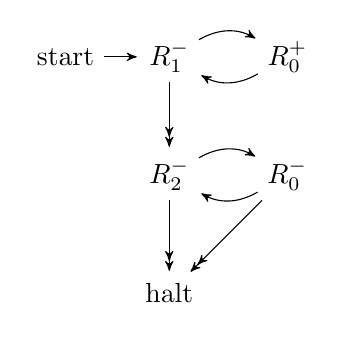
\begin{tikzpicture}
              \node[initial] (a) {$R_1^-$};
              \node (b) [right of=a] {$R_0^+$};
              \node (c) [below of=a] {$R_2^-$};
              \node (d) [right of=c] {$R_0^-$};
              \node (halt) [below of=c] {halt};

              \path
              (a) edge [bend left] (b)
              (b) edge [bend left] (a)
              (a) edge [->>] (c)
              (c) edge [bend left] (d)
              (d) edge [bend left] (c)
              (c) edge [->>] (halt)
              (d) edge [->>] (halt)
              ;
            \end{tikzpicture}
          \item
            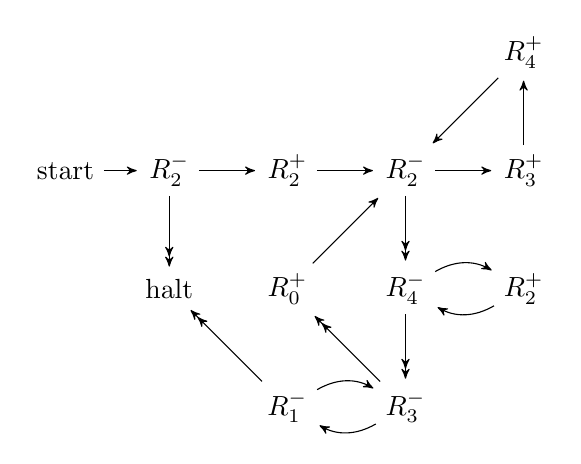
\begin{tikzpicture}
              \node[initial] (i) {$R_2^-$};
              \node (j) [right of=i] {$R_2^+$};
              \node (halt) [below of=i] {halt};

              \node (c) [right of=j] {$R_2^-$};
              \node (b) [right of=c] {$R_3^+$};
              \node (a) [above of=b] {$R_4^+$};

              \node (d) [below of=c] {$R_4^-$};
              \node (e) [right of=d] {$R_2^+$};

              \node (f) [below of=d] {$R_3^-$};
              \node (g) [left of=f] {$R_1^-$};

              \node (h) [above of=g] {$R_0^+$};

              \path
              (i) edge (j)
              (j) edge (c)
              (i) edge [->>] (halt)

              (c) edge (b)
              (b) edge (a)
              (a) edge (c)

              (c) edge [->>] (d)

              (d) edge [bend left] (e)
              (e) edge [bend left] (d)

              (d) edge [->>] (f)

              (f) edge [bend left] (g)
              (g) edge [bend left] (f)

              (f) edge [->>] (h)
              (h) edge (c)
              (g) edge [->>] (halt)
              ;
            \end{tikzpicture}
          \item
            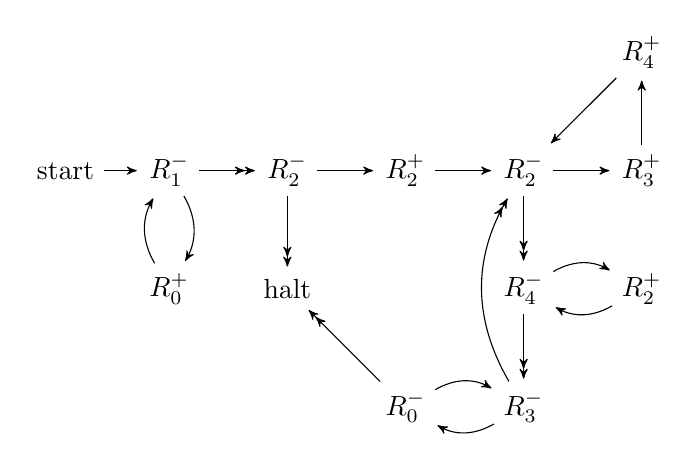
\begin{tikzpicture}
              \node[initial] (l) {$R_1^-$};
              \node (m) [below of=l] {$R_0^+$};

              \node (i) [right of=l] {$R_2^-$};
              \node (j) [right of=i] {$R_2^+$};
              \node (halt) [below of=i] {halt};

              \node (c) [right of=j] {$R_2^-$};
              \node (b) [right of=c] {$R_3^+$};
              \node (a) [above of=b] {$R_4^+$};

              \node (d) [below of=c] {$R_4^-$};
              \node (e) [right of=d] {$R_2^+$};

              \node (f) [below of=d] {$R_3^-$};
              \node (g) [left of=f] {$R_0^-$};

              \path
              (l) edge [bend left] (m)
              (m) edge [bend left] (l)

              (l) edge [->>] (i)

              (i) edge (j)
              (j) edge (c)
              (i) edge [->>] (halt)

              (c) edge (b)
              (b) edge (a)
              (a) edge (c)

              (c) edge [->>] (d)

              (d) edge [bend left] (e)
              (e) edge [bend left] (d)

              (d) edge [->>] (f)

              (f) edge [bend left] (g)
              (g) edge [bend left] (f)

              (f) edge [->>,bend left] (c)
              (g) edge [->>] (halt)
              ;
            \end{tikzpicture}
          \item
            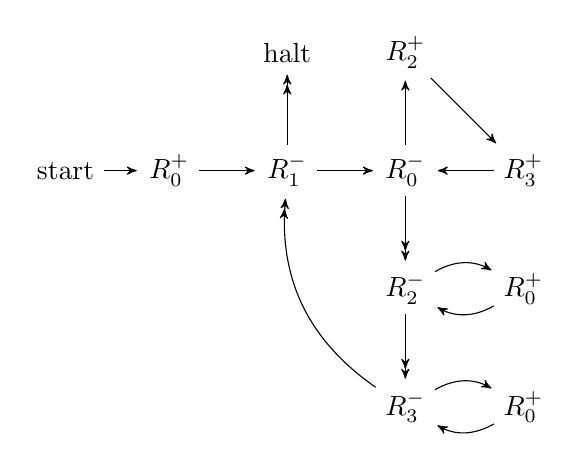
\begin{tikzpicture}
              \node[initial] (c) {$R_0^+$};
              \node (b) [right of=c] {$R_1^-$};
              \node (halt) [above of=b] {halt};

              \node (d) [right of=b] {$R_0^-$};
              \node (a) [above of=d] {$R_2^+$};
              \node (e) [right of=d] {$R_3^+$};

              \node (f) [below of=d] {$R_2^-$};
              \node (g) [right of=f] {$R_0^+$};

              \node (h) [below of=f] {$R_3^-$};
              \node (i) [right of=h] {$R_0^+$};

              \path
              (c) edge (b)
              (b) edge [->>] (halt)
                  edge (d)

              (d) edge (a)
                  edge [->>] (f)
              (a) edge (e)
              (e) edge (d)

              (f) edge [bend left] (g)
                  edge [->>] (h)
              (g) edge [bend left] (f)

              (h) edge [bend left] (i)
                  edge [->>,bend left] (b)
              (i) edge [bend left] (h)
              ;
            \end{tikzpicture}
          \item
            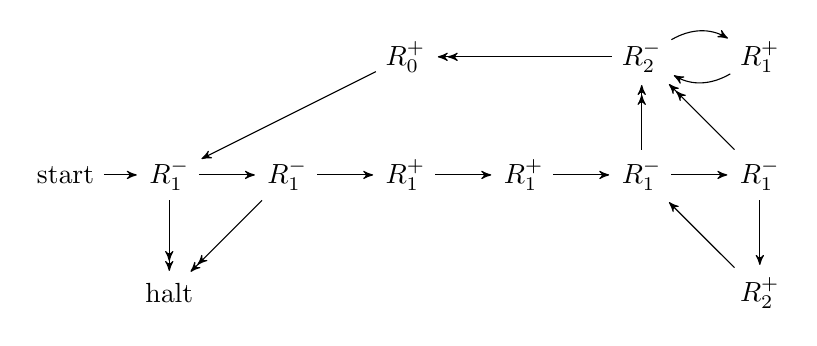
\begin{tikzpicture}
              \node[initial] (e) {$R_1^-$};
              \node (f) [right of=e] {$R_1^-$};
              \node (halt) [below of=e] {halt};

              \node (i) [right of=f] {$R_1^+$};
              \node (j) [right of=i] {$R_1^+$};

              \node (b) [right of=j] {$R_1^-$};
              \node (c) [right of=b] {$R_1^-$};
              \node (d) [below of=c] {$R_2^+$};

              \node (g) [above of=b] {$R_2^-$};
              \node (h) [right of=g] {$R_1^+$};

              \node (a) [above of=i] {$R_0^+$};

              \path
              (e) edge (f)
                  edge [->>] (halt)
              (f) edge (i)
                  edge [->>] (halt)
              (i) edge (j)
              (j) edge (b)
              (b) edge (c)
                  edge [->>] (g)
              (c) edge (d)
                  edge [->>] (g)
              (d) edge (b)

              (g) edge [bend left] (h)
                  edge [->>] (a)
              (h) edge [bend left] (g)

              (a) edge (e)
              ;
            \end{tikzpicture}
        \end{enumerate}
      \item The fact that $f$ is register machine computable means that there exists an $e$ such that $\phi_e=f$. An injection from register machines to register machines which preserves functionality is to add \texttt{HALT} instructions at the end of the program. This preserves functionality because, given original machine $M$, if $M$ had any jumps to the position of the new \texttt{HALT}, the machine would terminate immediately with an erroneous halt, but now terminates immediately with a proper halt. These are indistinguishable from the output of the machines. A machine with a different program has a different code, so we can add \texttt{HALT}s ad infinitum, producing infinitely many suitable $e$s, as required.
      \item The machine counts the number of times the value in $S$ can be divided by 2, putting the result in $A$.
    \end{enumerate}
  \item
    \lstinputlisting{s1.c}
    This is correct assuming that we have an infinite amount of addressable memory and that the machine never stores a register value outside the range of \texttt{unsigned int}. C libraries providing arbitrary size integers exist, and would provide a more correct implementation.
  \item C code can be compiled into assembly code. We can encode the memory of a computer as a list in one register of a register machine, and the assembly code can be encoded as a list in another register. The registers of the computer can be simulated as register machine registers, and in particular this includes the program counter.
  \item If we could test arbitrary programs for equality of outcome, we could test whether an arbitrary program $M$ halts on all inputs. To do this, we make $M$ return $0$ when it halts, then test whether $M$ is equal to the constant $0$ function. This solves the halting problem, and is thus contradictory. If we could number programs such that programs with the same outcome iff they have the same number, we would be able to test programs for this extensional equality.
  \item There are countably many possible register machines, and hence at most a countably infinite number of distinct computable functions. We know that $\mathbf N \to \mathbf N$ has strictly greater cardinality than $\mathbf N$, and hence strictly greater cardinality than the set of computable functions.
  \item As shown in question 1.2, there are infinitely many register machines to compute any function which is register machine computable. However, there are some normalizing operations which can be done on register machine programs, such as reducing to having one \texttt{HALT} at the end and removing increments followed by decrements in the same register. But we still have a similar problem as in question 4.
\end{enumerate}

\end{document}
